\documentclass[10pt,letterpaper]{article}
\usepackage[utf8]{inputenc}
\usepackage[spanish]{babel}
\usepackage{amsmath}
\usepackage{amsfonts}
\usepackage{amssymb}
\usepackage{graphicx}
\usepackage{float}

\graphicspath{ {img/} } 

\author{David Alejandro Castillo Chíquiza \\Sergio Esteban Triana Bobadilla \\David Alejandro Antolínez Socha}
\title{Taller 2 Grupo 2}

\begin{document}

\maketitle

\section{Punto 2}

	\subsection{Enunciado}
	
	Dado el sistema lineal de la forma $AX=b$ donde la matriz de coeficientes esta dado por:
	\begin{center}
	
		\begin{enumerate}
		
			\item[a)] Si $ A=\begin{bmatrix}4 & 3 & 0\\ 3 & 4 & -1 \\ 0 & -1 & 4 \end{bmatrix}$, es diagonalmente dominante.
			
			\item[b)] Calcule el radio espectral $\rho(\lambda)$ de la matriz de transición por el método de Gauss-Seidel.
			
			\item[c)] Utilice el método Gauss-Seidel para aproximar la solución con una tolerancia de $10^{-16}$, determine el numero de iteraciones. Tenga en cuenta que $$ b=\begin{bmatrix} 0.254 \\ -1.425 \\ 2.978  \end{bmatrix}$$
			
			\item[d)] Que pasa con la solución anterior si $a_{13}=-2$ explique su respuesta.
			
			\item[e)] Evalué matriz de transición del método \textbf{SOR} y determine varias soluciones aproximadas, para 10 valores de $w$. Utilice una tolerancia de $10^{-5}$.
		
		\end{enumerate}
		
	\end{center}
	
	\subsection{Solución}
		
	\begin{center}
	
		\begin{enumerate}
		
			\item[b)] El radio espectral es supremo de los valores absolutos dentro del espectro de una matriz
El proceso que se aplica para hallar este valor es el siguiente:\\
Suponiendo una matriz A, a la cual se descompondrá en 3 matrices, la matriz con su diagonal, la matriz con la triangular inferior y la matriz con la triangular superior.\\
lo siguiente que se realiza es hallar una matriz U restando la matriz de la diagonal a la matriz de la triangular superior, con esa matriz U se hace producto punto con la inversa de la matriz de la diagonal inferior y U y ese resultado se halla el máximo valor absoluto del espectro de la matriz.\\
			\begin{figure}[H]
				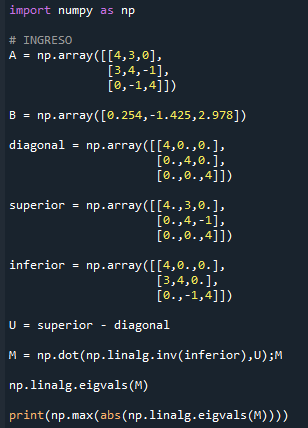
\includegraphics{imagen1}
				\centering
			\end{figure}
			
			\begin{figure}[H]
				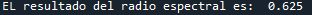
\includegraphics{imagen2}
				\centering
			\end{figure}
			\item[c)] Al aproximar la solución por el método de Gauss-Sediel la solución es la siguiente:
			\begin{figure}[H]
				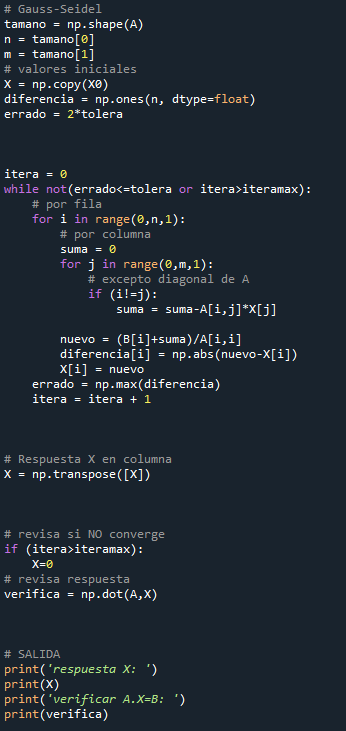
\includegraphics{imagen3}
				\centering
			\end{figure}
			\begin{figure}[H]
				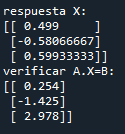
\includegraphics{imagen4}
				\centering
			\end{figure}
			Al final se hace la verificación, con el fin de corroborar que la solución si está correcta.
			\item[d)] Al aplicar el cambio dado $A_{13}=-2$, el resultado es el siguiente:\\
			\begin{figure}[H]
				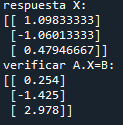
\includegraphics{imagen5}
				\centering
			\end{figure}
			podemos ver que con el cambio tenemos que la solución varía pasando de (0.499,-0.58066667,0.59933333) a (1.0983333,-1.06013333,0.47946667)
			\item[e)]
		\end{enumerate}
		
	\end{center}		
\section{Punto 7}
	
	\subsection{Enunciado}
	Dada la matriz $A$ (del punto 1) Verificar si:
	\begin{enumerate}
		\item[i.] Se puede descomponer de la forma LU, entonces utilice el resultado para resolver el sistema, teniendo en cuenta que la máquina admite cuatro dígitos significativos; ¿cómo afecta esto la respuesta?
	\end{enumerate}
	
	\subsection{Solución}
	Implementación del método para descomponer de la forma LU:\\
	\begin{figure}[H]
		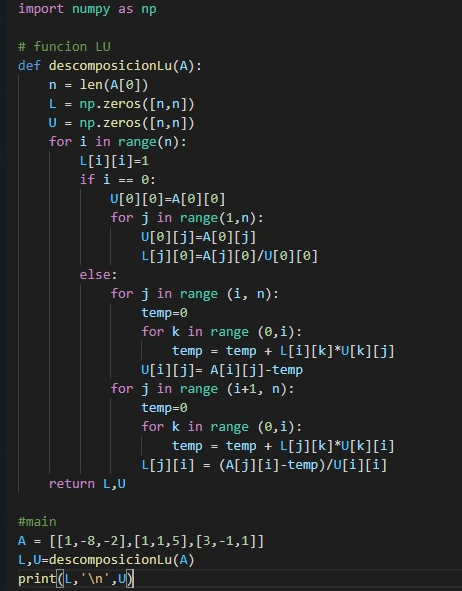
\includegraphics{imagen10}
		\centering
	\end{figure}
	Resultados de la implementación:\\
	\begin{figure}[H]
		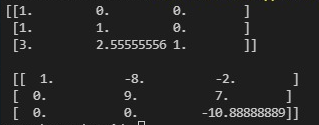
\includegraphics{imagen11}
		\centering
	\end{figure}	
	
\section{Punto 10}
	\subsection{Enunciado}
	Dado un sistema de ecuaciones no lineales, implemente el método de Newton Multivariado (es decir para varias variables) para resolver el problema:\\
	Determinar la intersección dela circunferencia $x^2+y^2=1$ y la recta $x=y$. Usamos una aproximación lineal $(1,1)$.
	\subsection{Solución}
	Implementación del metodo de Newton Multivariado:\\
	\begin{figure}[H]
		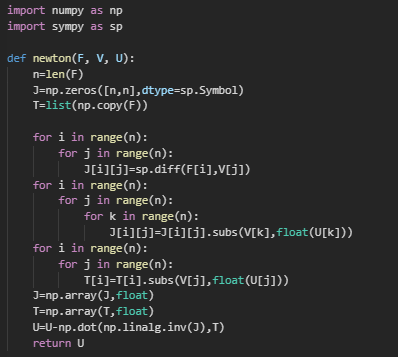
\includegraphics{imagen6}
		\centering
	\end{figure}
	Resultados de la implementación:\\
	\begin{figure}[H]
		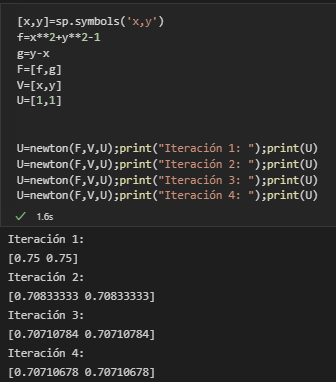
\includegraphics{imagen7}
		\centering
	\end{figure}
	Verficación en WolframAlpha:\\
	\begin{figure}[H]
		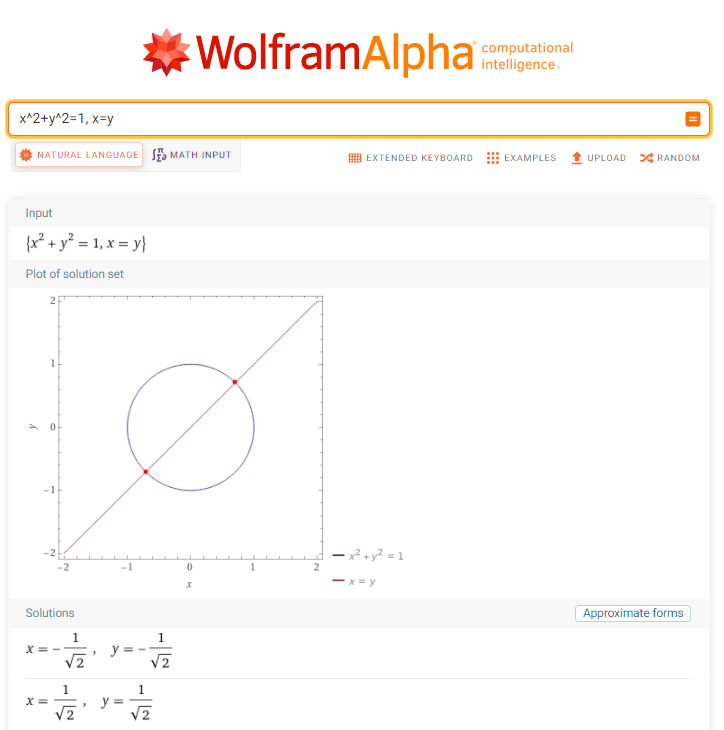
\includegraphics[width=\textwidth]{imagen8}
		\centering
	\end{figure}
	\begin{figure}[H]
		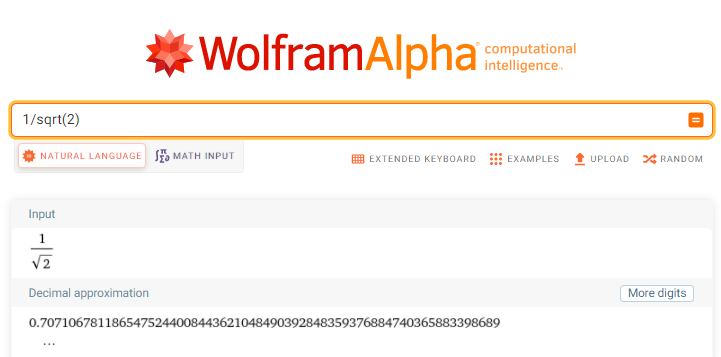
\includegraphics[width=\textwidth]{imagen9}
		\centering
	\end{figure}
	
\end{document}